\begin{figure}[!t]
\centering
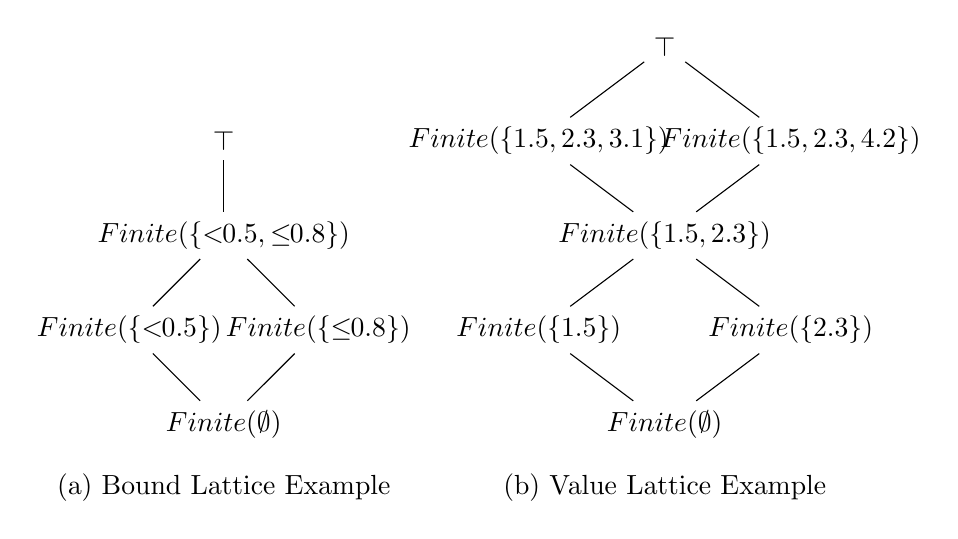
\begin{tikzpicture}[scale=0.8]
  % Individual lattice (left)
  \node (bot1) at (0,0) {$\text{Finite}(\emptyset)$};
  \node (s1) at (-1.5,1.5) {$\text{Finite}(\{<\!\!0.5\})$};
  \node (s2) at (1.5,1.5) {$\text{Finite}(\{\leq\!\!0.8\})$};
  \node (s12) at (0,3) {$\text{Finite}(\{<\!\!0.5, \leq\!\!0.8\})$};
  \node (top1) at (0,4.5) {$\top$};
  
  \draw (bot1) -- (s1);
  \draw (bot1) -- (s2);
  \draw (s1) -- (s12);
  \draw (s2) -- (s12);
  \draw (s12) -- (top1);
  
  \node at (0,-1) {(a) Bound Lattice Example};
  
  % Product lattice (right)
  \node (bot2) at (7,0) {$\text{Finite}(\emptyset)$};
  \node (s3) at (5,1.5) {$\text{Finite}(\{1.5\})$};
  \node (s4) at (9,1.5) {$\text{Finite}(\{2.3\})$};
  \node (s34) at (7,3) {$\text{Finite}(\{1.5, 2.3\})$};
  \node (s5) at (5,4.5) {$\text{Finite}(\{1.5, 2.3, 3.1\})$};
  \node (s6) at (9,4.5) {$\text{Finite}(\{1.5, 2.3, 4.2\})$};
  \node (top2) at (7,6) {$\top$};
  
  \draw (bot2) -- (s3);
  \draw (bot2) -- (s4);
  \draw (s3) -- (s34);
  \draw (s4) -- (s34);
  \draw (s34) -- (s5);
  \draw (s34) -- (s6);
  \draw (s5) -- (top2);
  \draw (s6) -- (top2);
  \node at (7,-1) {(b) Value Lattice Example};
\end{tikzpicture}
\caption{Lattice structure for float types. (a) shows an example bound lattice with comparison bounds. (b) the lattice over real values.}
\label{fig:lattice}
\end{figure}